\paragraph{QuizziPedia::Front-End::Views::FillingQuestionsView}
\begin{figure} [ht]
	\centering
	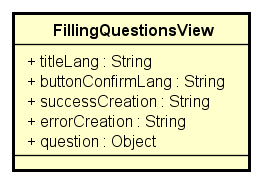
\includegraphics[scale=0.80]{UML/Classi/Front-End/QuizziPedia_Front-end_Views_FillingQuestionsView.png}
	\caption{QuizziPedia::Front-End::Views::FillingQuestionsView}
\end{figure} \FloatBarrier
\begin{itemize}
	\item \textbf{Descrizione}: view contenente i campi e le direttive per creare una domanda a riempimento testo;
	\item \textbf{Utilizzo}:  permette all'utente di creare una domanda a riempimento testo compilando i campi proposti;
	\item \textbf{Relazioni con altre classi}:
	\begin{itemize}
		\item \textit{IN} \texttt{FillingQuestionsModelView}: classe di tipo modelview la cui istanzazione è contenuta all'interno della variabile di ambiente \$scope di \texttt{Angular.js}. All'interno di essa sono presenti le variabili e i metodi necessari per il \textit{Two-Way Data-Binding\ped{G}} tra la view \texttt{FillingQuestionsView} e il controller \texttt{FillingQuestionsController};
		\item \textit{IN} \texttt{TopicKeywordsDirective}: directive che permette di gestire l'inserimento di keywords al momento della creazione della domanda;
		\item \textit{IN} \texttt{QuestionTextDirective}: rappresenta il componente grafico che permette all'utente di scrivere o modificare il testo di una domanda;
		\item \textit{IN} \texttt{LangModel}: rappresenta il modello delle informazioni per la giusta traduzione dell'applicazione.
	\end{itemize}
	\item \textbf{Attributi}:
	\begin{itemize}
		\item \texttt{+ question: Object} \\ Oggetto contenente gli attributi per la creazione della domanda:
		\begin{itemize}
			\item \texttt{answer}: array contenente oggetti che rappresentano le risposte. Ogni oggetto risposta contiene:
				\begin{itemize}
					\item \texttt{wordNumber}: attributo di tipo \texttt{Number} che indica la parola nel testo che andrà inserita in fase di compilazione.
				\end{itemize}
		\end{itemize}
		\item \texttt{+ titleLangFilling: String} \\ Attributo che viene utilizzato per visualizzare la giusta traduzione del titolo della pagina, in italiano o in inglese;
		\item \texttt{+ buttonConfirmLangFilling: String} \\ Attributo che viene utilizzato per visualizzare la giusta traduzione della \textit{label\ped{G}} per il bottone di conferma, in italiano o in inglese;
		\item \texttt{+ successCreation: String} \\ Attributo che visualizza un messaggio di conferma avvenuta creazione della domanda;
		\item \texttt{+ errorCreation: String} \\ Attributo che visualizza un messaggio d'errore per la creazione della domanda.
	\end{itemize}
\end{itemize}